\documentclass[unknownkeysallowed]{beamer}

\usepackage[utf8]{inputenc}
\usepackage[T1]{fontenc}
\usepackage[german]{babel}
\usepackage{graphicx} % Bilder
\usepackage{wrapfig} % Umflussbilder
\usepackage{multicol} % Multiple columns
\usepackage{minted} % Haskell source code
\usepackage{framed} % Frames around source code
\usepackage[framemethod=tikz]{mdframed} % Frames

\mdfdefinestyle{fancy}{
  roundcorner=5pt,
  linewidth=4pt,
  linecolor=red!80,
  backgroundcolor=red!20
}
\newmdenv[style=fancy]{important}

% Stuff for Beamer
\beamertemplatenavigationsymbolsempty
\usetheme{Warsaw}

\begin{document} 
  
%----------------------------------------------------------------------------------------  

  \begin{frame}
  %\begin{center}
    \huge\textbf{Fortgeschrittene funktionale Programmierung in Haskell}\\ \bigskip
    \LARGE Universität Bielefeld, Sommersemester 2015\\ \bigskip
    \large Jonas Betzendahl \& Stefan Dresselhaus
    %\end{center}
  \end{frame}

%----------------------------------------------------------------------------------------  
  
\begin{frame}
%\begin{center}
	\Large\textbf{\underline{Überblick für Heute:}}\bigskip \normalsize
	
	\begin{itemize}
	\item Organisatorisches \& Überlebenstipps
	\item Wiederholung Haskell-Basics
	\item Thinking in Types
	\item Lazy Evaluation
	\item Problemlösen durch Zusammenstecken
	\end{itemize}

%\end{center}
\end{frame}

%----------------------------------------------------------------------------------------  
  \section{Organisatorisches}
  
  \begin{frame}

    \begin{center}
    \Large\textbf{Organisatorisches \& Überlebenstipps}
    \end{center}
  \end{frame}

%----------------------------------------------------------------------------------------  
  
  \begin{frame}
    %\begin{center}
    \Large\textbf{Organisatorisches: Veranstaltungen}\bigskip \normalsize
    
    Es gibt Vorlesungen (Freitags, 14-16 Uhr in V2-205)\\
    und Übungen (Montags, 12-14 \& 18-20 Uhr in V2-221)\bigskip
	
	Teilnahme an den Übungen ist nicht verpflichtend, aber von Vorteil.  
    %\end{center}
  \end{frame}
  
%----------------------------------------------------------------------------------------  
  
  \begin{frame}
    %\begin{center}
    \Large\textbf{Organisatorisches (2): Input / Output}\bigskip \normalsize
    
    Das Modul gibt es 5 (echte) Leistungspunkte.\\
    Bürokratische Hürden $\Rightarrow$ LP nur für \emph{individuelle} Ergänzung \bigskip
    
    \textbf{Kriterium:} erfolgreicher Abschluss eines kleinen Programmierprojektes
    (Aufgabe TBA, Details in den Übungen)
    %\end{center}
  \end{frame}
  
%----------------------------------------------------------------------------------------  
  
  \begin{frame}
    %\begin{center}
    \Large\textbf{Organisatorisches (3): Personenkult}\bigskip \normalsize

	Wir, das sind Jonas Betzendahl und Stefan Dresselhaus.\\
	Mailadressen: \texttt{\{jbetzend,sdressel\}@techfak\dots}\\ \bigskip
    
    Formal verantwortlich:\\Dr. Alexander Sczyrba (\texttt{asczyrba@techfak\dots})
    
    (für Fragen im Kontext der Fakultät und Beschwerden zu uns)
    %\end{center}
  \end{frame}
  
%----------------------------------------------------------------------------------------  
  
  \begin{frame}
    %\begin{center}
	\Large\textbf{Organisatorisches (4): Material}\bigskip \normalsize
	
	Aufgabenblätter, Foliensätze, Beispiele, Vorlagen und sonstige Unterlagen entweder im ekVV oder zum Selberklonen auf GitHub:
	
	\bigskip\texttt{https://github.com/FFPiHaskell}\bigskip
	
	Audio \& Video - Mitschnitte auf YouTube, Näheres momentan ebenfalls TBA
    %\end{center}
  \end{frame}
  
%----------------------------------------------------------------------------------------  
  
  \begin{frame}
    %\begin{center}
    \Large\textbf{T \& R (1): Haskell / GHC}\bigskip \normalsize
    
    Standard in dieser Vorlesung ist der  \\ \texttt{Glasgow Haskell Compiler} (GHC)
    ($\geqslant$ v. 7.8, wo relevant) \pause \bigskip
    
    Rundum-Glücklich-Paket für eigene Rechner: \emph{Haskell Platform}\\
    \texttt{https://www.haskell.org/platform/} \pause \bigskip
    
    Aktuellen GHC (7.10) kriegt ihr im GZI mit dem rcinfo-Paket \texttt{ghc} \pause \smallskip
    
    \begin{important}
    \textbf{Wichtig:}\\Der Haskell-Interpreter \texttt{Hugs} wird von uns \underline{nicht} unterstützt!
    \end{important}
    %\end{center}
  \end{frame}
  
%----------------------------------------------------------------------------------------  
  
  \begin{frame}
    %\begin{center}
    \Large\textbf{T \& R (2): GHCi}\bigskip \normalsize
    
    Der GHC hat auch eine interaktive Umgebung: GHC\emph{I}.\\\bigskip
    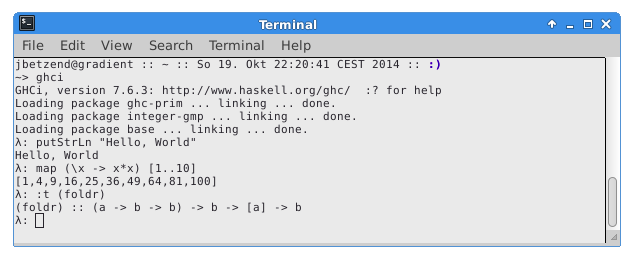
\includegraphics[scale=0.4]{ghci_example.png} 
    
    \bigskip GHCi bietet auch ein REPL (Read - Evaluate - Print - Loop),\\\emph{sehr} nützlich zum Entwickeln (ähnlich zu \texttt{Hugs}).
    %\end{center}
  \end{frame}
  
  %----------------------------------------------------------------------------------------  
  
  \begin{frame}
    %\begin{center}
    \Large\textbf{T \& R (3): Hackage}\bigskip \normalsize
    
    Die meisten Bibliotheken von Haskell wohnen auf \emph{Hackage}: \\ \bigskip \texttt{https://hackage.haskell.org/}
    
    Dort findet ihr übersichtliche Zusammenfassungen der Bibliotheken, detaillierte Auflistungen der exportierten Funktionen und Datentypen und die jeweiligen Implementationen (!).
    %\end{center}
  \end{frame}
  
%----------------------------------------------------------------------------------------  
  
  \begin{frame}
    %\begin{center}
    \Large\textbf{T \& R (4): cabal}\bigskip \normalsize
    
    Haskells \texttt{cabal} ist ein Programm zum erstellen, verpacken und installieren
    von Bibliotheken und Programmen:
    
    \begin{itemize}
    \item lokale Installation (keine sudo-Rechte notwendig)
    \item Zugriff auf Hackage 
    \item Hilfe beim Erstellen von Paketen
    \item Dependency management
    \item \dots
    \end{itemize}
    %\end{center}
  \end{frame}
  
%----------------------------------------------------------------------------------------  
  
  \begin{frame}
    %\begin{center}
    \Large\textbf{T \& R (5): LYAHFGG}\bigskip \normalsize
    
    \begin{multicols}{2}
    \begin{center}
	
\includegraphics[scale=0.15]{lyah.png} 
	\end{center}
	
	\columnbreak    
    Das Buch \glqq Learn You A Haskell\grqq\ ist die beste™ Ressource um die ersten 
    Schritte in Haskell zu lernen. \bigskip
   
    Ihr findet es online frei und kostenlos verfügbar hier:
    
    \texttt{http://learnyouahaskell.com/}
    \end{multicols}
    %\end{center}
  \end{frame}

%----------------------------------------------------------------------------------------  

\section{Wiederholung}
\begin{frame}
\begin{center}
\Large\textbf{Wiederholung Haskell-Basics}
\end{center}
\end{frame}

%----------------------------------------------------------------------------------------  
  
  \begin{frame}[fragile]
  
  %\begin{center}
  \Large\textbf{\underline{Haskell auf einer Folie:}} \bigskip \normalsize
  %\end{center}

  \begin{minted}[size=tiny]{haskell}
  -- Only those elements that conform to the predicate
  filter :: (a -> Bool) -> [a] -> [a]
  filter p []     = []
  filter p (x:xs) 
      | p x       = x : filter p xs
      | otherwise =     filter p xs
  \end{minted}
  
  \pause
  
  \begin{multicols}{2}
  \begin{itemize}
  \item Typsignaturen    \pause
  \item Pattern Matching \pause
  \item Polymorphismus   \pause
  \end{itemize}
  
  \columnbreak
  
  \begin{itemize}
  \item higher order fun. \pause
  \item Guards            \pause
  \item Curryfizierung    \pause
  \end{itemize}

  \end{multicols}
  

  \begin{itemize}
  \item Anwendung von Funktionen: \mint{haskell}|f x y -- statt f(x,y)|
  \end{itemize}
  
\end{frame}

%----------------------------------------------------------------------------------------  
\section{Thinking in Types}
\begin{frame}

    \begin{center}
    \Large\textbf{Thinking in Types}
    \end{center}

\end{frame}

%----------------------------------------------------------------------------------------  
  \subsection{Grundlagen}
  \begin{frame}[fragile]
  
  %\begin{center}
  \Large\textbf{\underline{Haskell auf \tiny etwas mehr als \,\Large einer Folie:}} \bigskip \normalsize
  %\end{center}
  
  Folgende Typen solltet ihr schon kennen...
  
  \begin{minted}[size=tiny]{haskell}
   Int, Integer, Float, Double, Char, String, Bool ...
  \end{minted}
  
  \pause
  
  ... außerdem gibt es Typkonstruktoren, die neue Typen machen ...
  
  \begin{minted}[size=tiny]{haskell}
   [], Tree, Maybe, Either, (,) ...
  \end{minted}
  
  \pause
  
  ... und so machen wir ganz neue Typen:

  \begin{minted}[size=tiny]{haskell}
   type List a = [a]
  \end{minted}
  
  \pause  
   
  \begin{minted}[size=tiny]{haskell}
   newtype Sekunden = Sekunden Int
  \end{minted}
  
  \pause
  
  \begin{minted}[size=tiny]{haskell}
   data Bool = False | True
   data [a]  = [] | a : [a] -- algebraisch, rekursiv
  \end{minted}
  
\end{frame}

%----------------------------------------------------------------------------------------  
  \subsection{Typklassen}
  \begin{frame}[fragile]
  
  \Large\textbf{Problemstellung:}\bigskip \normalsize

  Was ist das Problem mit folgender Funktion?

  \begin{minted}[size=tiny]{haskell}
   quadrat :: a -> a
   quadrat x = x * x
  \end{minted}
  
  \bigskip
  \pause
  
  $\to$ Funktion \texttt{(*)} könnte undefiniert für a sein (Funktionstypen) \\ \pause
  $\to$ Verschiedene Lösungsansätze: \pause
  
  \begin{itemize}
  \item \glqq Local choice\grqq , nur polymorphes Symbol (Abstraktionsverlust) \pause
  \item Standardimplementationen für Gleichheit etc. (Laufzeitfehler)
  \end{itemize}
\end{frame}

%----------------------------------------------------------------------------------------  
  
  \begin{frame}[fragile]
  
  \Large\textbf{Haskell-Lösung: Typklassen} \normalsize

  \begin{minted}[size=tiny]{haskell}
   quadrat :: Num a => a -> a
   quadrat x = x * x
  \end{minted}
  
  Polymorphismus beschränkt auf die Typen, die auch bestimmte Funktionen unterstützen.\pause  
  \begin{multicols}{2}
  \emph{Abstrakte Definition:}
  
  \begin{minted}[size=tiny]{haskell}
class Num a where
  (+)    :: a -> a -> a
  (*)    :: a -> a -> a
  negate :: a -> a
  ...
  \end{minted}

  \vfill \vfill  
  
  \pause
  \columnbreak  
  \emph{Konkrete Instanz:}
  
  \begin{minted}[size=tiny]{haskell}
instance Num Int where
  i + j    = plusInt i j
  i * j    = mulInt  i j 
  negate i = negInt  i
  ... 
  \end{minted}
  \pause
  \texttt{plusInt, mulInt} und \texttt{negInt} an anderer Stelle definiert.
  \end{multicols}  
  
\end{frame}

%----------------------------------------------------------------------------------------  
  
  \begin{frame}[fragile]
  
  Es gibt in Haskell zwei Möglichkeiten, einen Typen einer Typklasse hinzuzufügen:\pause  
  
  \begin{multicols}{2}
  \emph{Von Hand:}
  
  \begin{minted}[size=tiny]{haskell}
  class Show a where
   show :: a -> String
  
  data Bool = False | True

  instance Show Bool where
    show False = "False"
    show True  = "True"
  \end{minted}
  
  \pause
  \columnbreak  
  \emph{Automatisch:}
  
  \begin{minted}[size=tiny]{haskell}
  class Show a where
    show :: a -> String  
  
  data Bool = False | True 
              deriving Show
  \end{minted}
  \end{multicols} 
  
\end{frame}

%----------------------------------------------------------------------------------------  

  \begin{frame}[fragile]
  
  Weitere Beispiele für Typklassen: \pause

  \begin{minted}[size=tiny]{haskell}
class Eq a where
  (==) :: a -> a -> Bool        -- minimal definition
  ...
  \end{minted}
  
  \pause
  
  \begin{minted}[size=tiny]{haskell}
class Eq a => Ord a where
  (<=)    :: a -> a -> Bool     -- minimal definition
  compare :: a -> a -> Ordering -- data Ordering=LT|EQ|GT
  ...
  \end{minted}
  
  \pause
  
  \begin{minted}[size=tiny]{haskell}
class Show a where
  show :: a -> String           -- minimal definition
  \end{minted}
  
  \pause
  
  $\Rightarrow$ Mehr zu Typklassen (inkl. \texttt{Functor, Applicative, Monad}) 
  nächste Woche.

\end{frame}

%----------------------------------------------------------------------------------------

\subsection{Purity}
\begin{frame}

    \begin{center}
    \Large\textbf{Purity}
    \end{center}

\end{frame}

%----------------------------------------------------------------------------------------
  
\section{Lazy Evaluation}
\begin{frame}

    \begin{center}
    \Large\textbf{Lazy Evaluation}
    \end{center}

\end{frame}

%----------------------------------------------------------------------------------------  

  \begin{frame}[fragile]

  \begin{minted}[size=tiny]{haskell}
        -- ... to be implemented
  \end{minted}
\end{frame}
  

\end{document}